\documentclass[10pt]{beamer}
\usepackage{amsmath,amsthm,mathtools,amssymb}
\usepackage{quantikz}

\title[QEC]{Quantum Error Correction - Stabiliser Codes}
\subtitle{PHYS650 Presentation}
\author[DP]{Dhawal Patil}
\date[12-09-25]{Dec 09 2025}

\begin{document}

\begin{frame}
	\titlepage
\end{frame}

\begin{frame} {No cloning theorem}
	Quantum states can not be freely copied
\begin{align*}
	A( \alpha \ket{0} + \beta \ket{1} ) 
	={}& ( \alpha \ket{0} + \beta \ket{1})( \alpha \ket{0} + \beta \ket{1})  \\
	={}& \alpha^2 \ket{00} + \alpha \beta \ket{01} + \alpha \beta \ket{10} + \beta^2 \ket{11} \\
	\not ={}& \alpha \ket{00} + \beta \ket{11} \\
	={}& \alpha A \ket{0} + \beta A \ket{1}
\end{align*}
\end{frame}


\begin{frame}[allowframebreaks] {Two qubit detection algorithm}
\begin{enumerate}
\item $$ \psi = \alpha \ket{0} + \beta \ket{1} \xrightarrow{\text{two qubit encoder}}
	\alpha \ket{00} + \beta \ket{11} .$$
\item Code space = $ \mathcal{C} = span\{  \ket{00}, \ket{11} \}.$
\item Error space $ \mathcal{F} = span \{ \ket{01}, \ket{10} \}.$
\item For stabilisers $$ Z_1 Z_2 
	= \begin{bmatrix}
		1 & 0 & 0 & 0 \\
		0 & -1 & 0 & 0 \\
		0 & 0 & -1 & 0 \\
		0 & 0 & 0 & 1
	\end{bmatrix} ,$$
	$Z_1 Z_2 \psi = - \psi$ if there is an error and $\psi$ if there is no error.
\pagebreak
\item  To extract this information, use a syndrome qubit
	$s$
\begin{figure}
	\begin{quantikz}
		\psi & \gate{E} &
		\gate{{Z_1 Z_2}} & \\
		\lstick{\ket{0}} & \gate{H} & \ctrl{-1}
				 & \gate{H} & \meter{} 
	\end{quantikz}
\end{figure}
\item If there was an error, then the transition would be
	$$ \psi \ket{+} \to - \psi \ket{-} \to - \psi \ket{1} $$
\item In a nutshell, states from $\mathcal{F}$ return a characteristic value of $-1$ and this can be 
	read from the syndrome qubit.
\item From $\ket{01}$ or $\ket{10},$ we can't go back to the original state. \textbf{Detection only}
\end{enumerate}
\end{frame}

\begin{frame}
	{Stabiliser Codes}
\begin{enumerate}
	\item Split the space into $\mathcal{C}$ Codespace and error subspaces $\mathcal{F}_i$
	one for each type of error.
\item Stabiliser group $S$ is a subgroup of $\mathcal{G}_n.$
\item $S$ stabilises $\mathcal{C},$ so it is in the subspace corresponding to $1$
\item $\mathcal{F}_i$ is in characteristic subspace corresponding  $-1.$
\end{enumerate}
\end{frame}

	
\begin{frame} [fragile] {Two Qubit Detection Code}
\begin{enumerate}
	\item All errors are unitary, so can be reversed by applying $E ^\dagger.$
\item The circuit
	\item $d = 2$ Indeed, replacing the first and third bits on $\ket{0110}$ yields $\ket{1100}.$
		So, $t = \lfloor \frac{d}{2} \rfloor = 0$ errors can be corrected.
		\item \textbf{Detection only}
\end{enumerate}	
\begin{figure}[h]
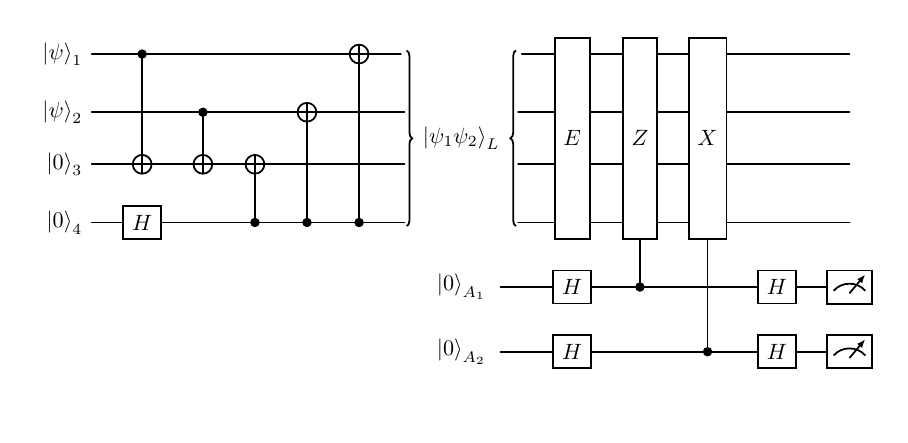
\begin{tikzpicture}
	\node[scale = 0.8]{
	\begin{quantikz}
	\lstick{ $ \ket{ \psi}_1 $ } & \ctrl{2} & & & & \targ{} 
	     & \midstick[4] { $ \ket{ \psi_1 \psi_2} _L $ }
	     & \gate[4] {E} 
	     &
	     \gate[4] { Z }
	     & 
	     \gate[4] {
		     X
	     }
	     & & \\
	\lstick{ $ \ket{ \psi}_2 $ } & & \ctrl{1} & & \targ{} & 
	     & & 
	     & & & & \\
	\lstick{ $ \ket{0}_3 $ } & \targ{} & \targ{} & \targ {} & & 
		 & & & & & & \\
	\lstick{ $ \ket{0}_4 $ } & \gate{H} & & \ctrl{-1} & \ctrl{-2} & \ctrl{-3} 
				 & & & & & & \\
	\setwiretype{n} & & & & & &
	\midstick{$ \ket{0}_{A_1} $} & \gate{H} \setwiretype{q} & \ctrl{-4} & & \gate{H} & \meter{} \\
	\setwiretype{n} & & & & & &
	\midstick{$ \ket{0}_{A_2} $} & \gate{H} \setwiretype{q} & & \ctrl{-4} & \gate{H} & \meter{} \\
\end{quantikz}
};
\end{tikzpicture}
\end{figure}

\end{frame}

\begin{frame}
\begin{enumerate}
	\item For an $(n, k, d)$ code, $k$ logical qubits can be encoded into $n$ physical qubits.
	\item Efficiency of encoding is $k/n.$
	\item On propagation of $1$ error, a state can enter one of 
\end{enumerate}
\end{frame}

\begin{frame}
	{Stabiliser Codes}
\begin{enumerate}
\item {The $[[ 5,1,3 ]]$ Code}
	Capable of correcting all kinds of errors on one logical qubit.
\item Stabiliser Codes [BAD] - higher dimension codes have denser parity checks,
	more susceptible to decoherence
\item Alternate - Low Density Parity Check Code
\item Stabiliser Codes [BAD] - difficult to find stabiliser subgroups
\item Alternate - Surface code
\end{enumerate}
\end{frame}

\begin{frame}{Surface Codes}
\begin{enumerate}
    \item Surface codes belong to a class of topological stabiliser codes.
    \item Qubits arranged on a 2-D lattice. Stabiliser checks are local.
    \item Two types of checks:
        \begin{itemize}
            \item Star operators (measure $X$-type parity)
            \item Plaquette operators (measure $Z$-type parity)
        \end{itemize}
    \item Errors create ``defects’’ which appear as flipped stabiliser values.
    \item Decoding = finding a minimal path that connects these defects.
    \item Pros:
        \begin{itemize}
            \item Very high threshold ($\sim 1\%$)
            \item Only nearest-neighbour interactions needed
        \end{itemize}
    \item Cons:
        \begin{itemize}
            \item Very large number of physical qubits needed per logical qubit.
        \end{itemize}
\end{enumerate}
\end{frame}


\begin{frame}{Low Density Parity Check (LDPC) Codes}
\begin{enumerate}
    \item LDPC codes have stabilisers that touch only a small number of qubits.
    \item Sparse parity check matrix $\Rightarrow$ fewer operations per check.
    \item Pros:
        \begin{itemize}
            \item Much lower overhead than surface codes.
            \item Potential for constant-rate quantum codes (good $k/n$).
            \item Can achieve good distances without huge lattices.
        \end{itemize}
    \item Cons:
        \begin{itemize}
            \item Hard to find LDPC codes that also allow easy decoding.
            \item Harder to implement on hardware due to non-local checks.
        \end{itemize}
    \item Active research area: quantum expander codes, hypergraph product codes.
\end{enumerate}
\end{frame}


\begin{frame}
	{References}
	\bibliography{myref.bib}
	\cite{roffe}
\end{frame}


\end{document}

